\documentclass[a4paper,11pt]{article}
\usepackage[utf8]{inputenc}
\usepackage{minted}
\usepackage{amsmath}
\usepackage{float}
\usepackage[symbol]{footmisc}
\usepackage{graphicx}
\usepackage[toc,page]{appendix}

\graphicspath{{./figures/}}
\renewcommand{\thefootnote}{\fnsymbol{footnote}}

\title{\textbf{3. Sorting}}
\author{Kristiāns Vinters}
\date{Fall 2023}

\begin{document}
    \maketitle
    \section*{Introduction}

    I solved the sorted array search assignment in Go. I used Go because I want to become more familiar with it. Source code and benchmark data is available on GitHub\footnote[1]{https://github.com/Phanty133/id1021/tree/master/3-sorting}.

    \section*{Implementation}

    There weren't any particular difficulties in implementing the search algorithms in Go. The implementations are very similar to the given Java examples. The only difficulty I faced was when I forgot to make a copy of the pre-sorted array, as the arrays are sorted in-place. This oversight created nonsensical results, which showed insertion sort being significantly faster than merge sort. The reason for this is that insertion sort has less overhead and is significantly faster on already sorted arrays than merge sort.

    \section*{Benchmarking}

    I benchmarked the sorting algorithms by running them 10 times on 100 different, randomly generated integer arrays for array sizes 100, 1000, 2500, 5000, 10000, 25000, 50000, $75000^\dagger$, $100000^\dagger$, 250000\footnote[2]{Only insertion, merge, and merge2 sort were tested. The tests were done on 10 different arrays with 10 times.}.
    The benchmark function implementation is given in appendix \ref{appendix:benchmark}. All benchmarks were run on a Ryzen 5 5600H CPU with 16GB of RAM.

    The benchmark results show that, generally, selection sort is slower than insertion sort, which in turn is slower than merge sort.


    \begin{figure}[H]
        \centering
        
        \begin{tabular}{c|c|c|c|c}
            Size & $t_\text{Selection}$, ms & $t_\text{Insertion}$, ms & $t_\text{Merge}$, ms & $t_\text{Merge 2}$, ms \\
            \hline
            \hline
            100 & 0.006 & 0.003 & 0.003 & 0.003 \\
            \hline
            1000 & 0.470 & 0.130 & 0.046 & 0.040 \\
            \hline
            5000 & 9.60 & 3.11 & 0.293 & 0.257 \\
            \hline
            50000 & 930 & 330 & 3.65 & 3.29 \\
            \hline
            100000 & N/A & 1320 & 7.78 & 5.11 \\
            \hline
            250000 & N/A & 8330 & 20.4 & 18.4 \\
        \end{tabular}

        \caption{Subset of median times for sorting algorithms. Full results available on the GitHub repository.}
    \end{figure}

    \begin{figure}[H]
        \centering
        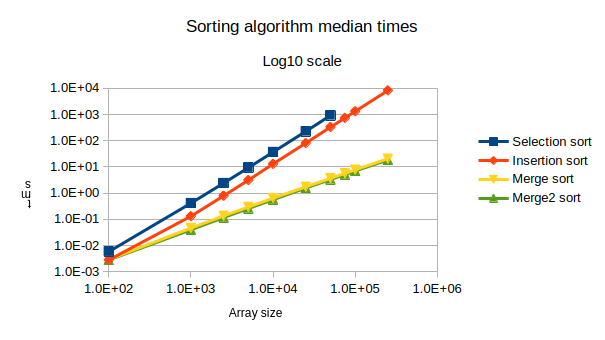
\includegraphics[width=\textwidth]{sorting.png}
        \caption{Benchmark results for sorting algorithms.}
        \label{fig:sorting}
    \end{figure}

    As expected, as the array size increases, both merge sort implementation median execution times grow slower than for insertion or selection sort. Using the selection sort times as a reference, we can see that insertion sort has a consistent ratio vs selection sort, while the ratio for merge sort significantly increases over array size. This is because selection and insertion sort is $O(n^2)$, while merge sort is $O(n \log n)$ on average.

    \begin{figure}[H]
        \centering
        \begin{tabular}{c|c|c|c}
            Size & Insertion & Merge & Merge 2 \\
            \hline
            \hline
            100 & 2.1 & 2.0 & 2.1 \\
            \hline
            1000 & 3.1 & 8.9 & 10.4 \\
            \hline
            5000 & 3.0 & 31.7 & 36.2 \\
            \hline
            50000 & 2.8 & 251.7 & 279.9 \\
        \end{tabular}

        \caption{Ratio of median times for sorting algorithms vs selection sort $\frac{t_{\text{Selection}}}{t_{\left\{\text{Insertion}, \text{Merge}, \text{Merge 2}\right\}}}$}
    \end{figure}

    The following figures (Fig. \ref{fig:n2} and \ref{fig:nlogn}) confirm the $O(n^2)$ and $O(n \log n)$ time complexities for selection, insertion and merge sort, respectively.

    \begin{figure}[H]
        \centering
        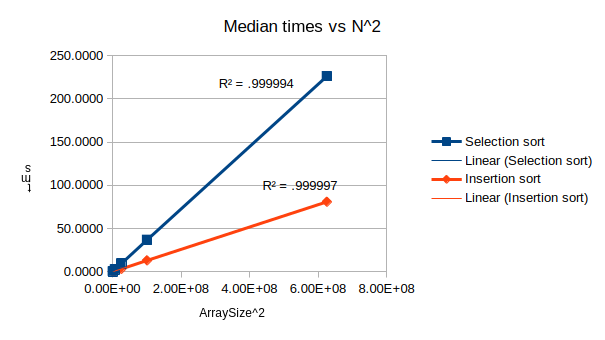
\includegraphics[width=\textwidth]{n2.png}
        \caption{Selection and insertion sort median times vs $\text{ArraySize}^2$}
        \label{fig:n2}   
    \end{figure}

    \begin{figure}[H]
        \centering
        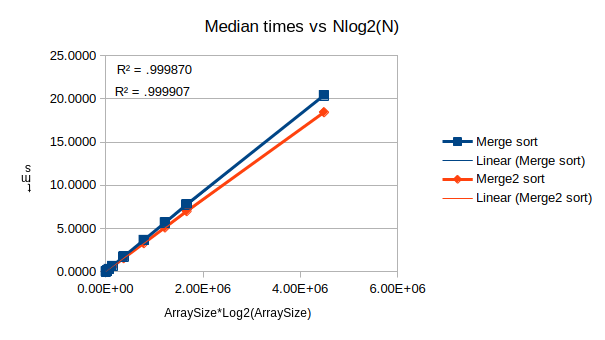
\includegraphics[width=\textwidth]{nlogn.png}
        \caption{Merge sort median times vs $\text{ArraySize}\cdot\log_2{\left(\text{ArraySize}\right)}$}
        \label{fig:nlogn}   
    \end{figure}

    The benchmarks also show a slight difference between the two merge sort implementations. Both implementations are still $O(n \log n)$, but the second implementation has slightly lower constant factors due to it doing less copying. The performance improvement is around $12\%$ overall, but it appears to reduce to around $11\%$ as the array size increases.

    \begin{figure}[H]
        \centering
        \begin{tabular}{c|c}
            Size & Ratio \\
            \hline
            \hline
            100 & 1.05 \\
            \hline
            1000 & 1.16 \\
            \hline
            5000 & 1.14 \\
            \hline
            50000 & 1.11 \\
            \hline
            100000 & 1.11 \\
            \hline
            250000 & 1.11 \\
        \end{tabular}

        \caption{Ratio $\frac{t_{\text{Merge}}}{t_{\text{Merge 2}}}$ for median times}
        \label{fig:merge}
    \end{figure}

    \begin{figure}[H]
        \centering
        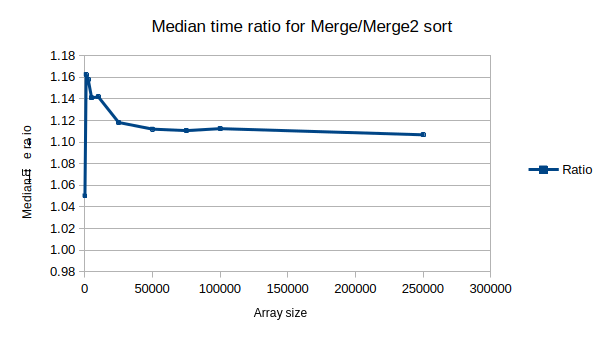
\includegraphics[width=\textwidth]{ratio.png}
        \caption{Ratio $\frac{t_{\text{Merge}}}{t_{\text{Merge 2}}}$ for median times}
        \label{fig:ratio}
    \end{figure}

    \begin{appendices}
        \section{Benchmark}
        \label{appendix:benchmark}
        \begin{minted}{go}
func BenchSort(
    sort func([]int),
    benchArrays [][]int,
    n, max, repeats int
) [][]float64 {
    times := make([][]float64, len(benchArrays))

    for i, arr := range benchArrays {
        times[i] = make([]float64, repeats)

        for r := 0; r < repeats; r++ {
            arrCopy := make([]int, len(arr))
            copy(arrCopy, arr)

            start := time.Now()
            sort(arrCopy)
            elapsed := time.Since(start)

            times[i][r] = float64(elapsed.Nanoseconds()) / 1000 / 1000
        }
    }

    return times
}
        \end{minted}
    \end{appendices}
\end{document}
